%Version 2.1 April 2023
% See section 11 of the User Manual for version history
%
%%%%%%%%%%%%%%%%%%%%%%%%%%%%%%%%%%%%%%%%%%%%%%%%%%%%%%%%%%%%%%%%%%%%%%
%%                                                                 %%
%% Please do not use \input{...} to include other tex files.       %%
%% Submit your LaTeX manuscript as one .tex document.              %%
%%                                                                 %%
%% All additional figures and files should be attached             %%
%% separately and not embedded in the \TeX\ document itself.       %%
%%                                                                 %%
%%%%%%%%%%%%%%%%%%%%%%%%%%%%%%%%%%%%%%%%%%%%%%%%%%%%%%%%%%%%%%%%%%%%%

%%\documentclass[referee,sn-basic]{sn-jnl}% referee option is meant for double line spacing

%%=======================================================%%
%% to print line numbers in the margin use lineno option %%
%%=======================================================%%

%%\documentclass[lineno,sn-basic]{sn-jnl}% Basic Springer Nature Reference Style/Chemistry Reference Style

%%======================================================%%
%% to compile with pdflatex/xelatex use pdflatex option %%
%%======================================================%%

%%\documentclass[pdflatex,sn-basic]{sn-jnl}% Basic Springer Nature Reference Style/Chemistry Reference Style


%%Note: the following reference styles support Namedate and Numbered referencing. By default the style follows the most common style. To switch between the options you can add or remove “Numbered” in the optional parenthesis. 
%%The option is available for: sn-basic.bst, sn-vancouver.bst, sn-chicago.bst, sn-mathphys.bst. %  
 
%%\documentclass[sn-nature]{sn-jnl}% Style for submissions to Nature Portfolio journals
%%\documentclass[sn-basic]{sn-jnl}% Basic Springer Nature Reference Style/Chemistry Reference Style
%\documentclass[sn-mathphys,Numbered]{sn-jnl}% Math and Physical Sciences Reference Style
%%\documentclass[sn-aps]{sn-jnl}% American Physical Society (APS) Reference Style
%%\documentclass[sn-vancouver,Numbered]{sn-jnl}% Vancouver Reference Style
\documentclass[sn-apa]{sn-jnl}% APA Reference Style 
%%\documentclass[sn-chicago]{sn-jnl}% Chicago-based Humanities Reference Style
%%\documentclass[default]{sn-jnl}% Default
%%\documentclass[default,iicol]{sn-jnl}% Default with double column layout

%%%% Standard Packages
%%<additional latex packages if required can be included here>

\usepackage{graphicx}%
\usepackage{multirow}%
\usepackage{amsmath,amssymb,amsfonts}%
\usepackage{amsthm}%
\usepackage{mathrsfs}%
\usepackage[title]{appendix}%
\usepackage{xcolor}%
\usepackage{textcomp}%
\usepackage{manyfoot}%
\usepackage{booktabs}%
\usepackage{algorithm}%
\usepackage{algorithmicx}%
\usepackage{algpseudocode}%
\usepackage{listings}%
%%%%

%%%%%=============================================================================%%%%
%%%%  Remarks: This template is provided to aid authors with the preparation
%%%%  of original research articles intended for submission to journals published 
%%%%  by Springer Nature. The guidance has been prepared in partnership with 
%%%%  production teams to conform to Springer Nature technical requirements. 
%%%%  Editorial and presentation requirements differ among journal portfolios and 
%%%%  research disciplines. You may find sections in this template are irrelevant 
%%%%  to your work and are empowered to omit any such section if allowed by the 
%%%%  journal you intend to submit to. The submission guidelines and policies 
%%%%  of the journal take precedence. A detailed User Manual is available in the 
%%%%  template package for technical guidance.
%%%%%=============================================================================%%%%

%\jyear{2021}%

%% as per the requirement new theorem styles can be included as shown below
\theoremstyle{thmstyleone}%
\newtheorem{theorem}{Theorem}%  meant for continuous numbers
%%\newtheorem{theorem}{Theorem}[section]% meant for sectionwise numbers
%% optional argument [theorem] produces theorem numbering sequence instead of independent numbers for Proposition
\newtheorem{proposition}[theorem]{Proposition}% 
%%\newtheorem{proposition}{Proposition}% to get separate numbers for theorem and proposition etc.

\theoremstyle{thmstyletwo}%
\newtheorem{example}{Example}%
\newtheorem{remark}{Remark}%

\theoremstyle{thmstylethree}%
\newtheorem{definition}{Definition}%

\raggedbottom
%%\unnumbered% uncomment this for unnumbered level heads

\begin{document}

\title[Decomposing a Sullivan expectancy: An indirect incidence-based
approach]{Decomposing a Sullivan expectancy: An indirect incidence-based
approach}

%%=============================================================%%
%% Prefix	-> \pfx{Dr}
%% GivenName	-> \fnm{Joergen W.}
%% Particle	-> \spfx{van der} -> surname prefix
%% FamilyName	-> \sur{Ploeg}
%% Suffix	-> \sfx{IV}
%% NatureName	-> \tanm{Poet Laureate} -> Title after name
%% Degrees	-> \dgr{MSc, PhD}
%% \author*[1,2]{\pfx{Dr} \fnm{Joergen W.} \spfx{van der} \sur{Ploeg} \sfx{IV} \tanm{Poet Laureate} 
%%                 \dgr{MSc, PhD}}\email{iauthor@gmail.com}
%%=============================================================%%

\author*[1,2]{\fnm{Tim} \sur{Riffe}}\email{tim.riffe@ehu.eus}

\author[1]{\fnm{Rustam} \sur{Tursun-zade}}\email{rustam.tursunzade@ehu.eus }
\equalcont{These authors contributed equally to this work.}

\affil*[1]{\orgdiv{OPIK, Department of Sociology and Social Work}, \orgname{University of the Basque Country (UPV/EHU)}, \orgaddress{\street{Barrio de Sarriena s/n }, \city{Leioa}, \postcode{48940},  \country{Spain}}}

\affil[2]{\orgname{Ikerbasque (Basque Foundation for Science}, \orgaddress{\street{Plaza Euskadi 5}, \city{Bilbao}, \postcode{48009},  \country{Spain}}}

%%==================================%%
%% sample for unstructured abstract %%
%%==================================%%

\abstract{\textbf{Background}: A lifetable and the prevalence of some health
condition are sufficient to calculate a health expectancy (HLE) using
the Sullivan method \citep{sullivan1971single}, and there are methods available
to decompose differences in HLE \citep{nusselder2004decomposition, shkolnikov2017decomposition}. But you still might not be
satisfied because observed prevalence could be driven by unobserved
mortality differences by health state, and because the lifetable is
itself a prevalence-weighted average of the mortality by different
health states. Thus these decomposition methods are not guaranteed to
isolate health and mortality effects.

\textbf{Objectives}: We aim to (i) transform Sullivan inputs into
state-specific mortality schedules consistent with a given mortality
rate ratio, and to (ii) convert prevalence into incidence for the case
of health deterioration without possibility of recovery. These rates can
be considered independent of one another, allowing for rate-based
decomposition and a cleaner separation of health and mortality effects.

\textbf{Methods}: Our approach is premised on an algebraic
transformation of mortality, prevalence, and an imposed all-cause
mortality rate-ratio between states (which might come from the
literature). Transition probabilities representing health deterioration
are then inferred following the logic of multistate lifetable
accounting. We first derive discrete-time transition probabilities, then
we reframe the calculation of health expectancy in terms of these. All
resulting expectancies (total and for states) are identical to the
traditional Sullivan one, but corresponding decomposition results are
now based on incidence parameters.

\textbf{Results}: Both marginal sums and age patterns attributable to
health and mortality differences are different when we decompose using
the indirectly derived multistate expectancies versus a standard
Sullivan decomposition. Interestingly, this method also enables a new
decomposition of total life expectancy that includes a health component.

\textbf{Conclusions}: This method gives an indirect method to transform
Sullivan-style inputs into a simple multistate model with an
irreversible health state, and then shows how to decompose expectancies
in terms of these new parameters. This might seem hypothetical because
we do not observe a mortality rate ratio, but we think even so it's more
informative than previously proposed Sullivan decompositions.
}

%%================================%%
%% Sample for structured abstract %%
%%================================%%

% \abstract{\textbf{Purpose:} The abstract serves both as a general introduction to the topic and as a brief, non-technical summary of the main results and their implications. The abstract must not include subheadings (unless expressly permitted in the journal's Instructions to Authors), equations or citations. As a guide the abstract should not exceed 200 words. Most journals do not set a hard limit however authors are advised to check the author instructions for the journal they are submitting to.
% 
% \textbf{Methods:} The abstract serves both as a general introduction to the topic and as a brief, non-technical summary of the main results and their implications. The abstract must not include subheadings (unless expressly permitted in the journal's Instructions to Authors), equations or citations. As a guide the abstract should not exceed 200 words. Most journals do not set a hard limit however authors are advised to check the author instructions for the journal they are submitting to.
% 
% \textbf{Results:} The abstract serves both as a general introduction to the topic and as a brief, non-technical summary of the main results and their implications. The abstract must not include subheadings (unless expressly permitted in the journal's Instructions to Authors), equations or citations. As a guide the abstract should not exceed 200 words. Most journals do not set a hard limit however authors are advised to check the author instructions for the journal they are submitting to.
% 
% \textbf{Conclusion:} The abstract serves both as a general introduction to the topic and as a brief, non-technical summary of the main results and their implications. The abstract must not include subheadings (unless expressly permitted in the journal's Instructions to Authors), equations or citations. As a guide the abstract should not exceed 200 words. Most journals do not set a hard limit however authors are advised to check the author instructions for the journal they are submitting to.}

\keywords{Healthy, Mortality, Prevalence, Incidence, Decomposition}

%%\pacs[JEL Classification]{D8, H51}

%%\pacs[MSC Classification]{35A01, 65L10, 65L12, 65L20, 65L70}

\maketitle

\section{Introduction}\label{sec1}


Healthy life expectancy (HLE, also called healthy life years) is most often calculated and reported using the Sullivan method \citep{sullivan1971single}, and often the resulting estimate is very close to what would be derived from a multistate model. It's only natural for a demographer to want to decompose a Sullivan-derived expectancies. Decomposition tells us what drives the differences, and has the potential to better guide efforts to improve health and longevity. The parameters of a Sullivan estimate are a single lifetable and information on the prevalence of a health condition. Decomposition approaches that have thus far been proposed include the widely-used \citet{nusselder2004decomposition} approach, which frames mortality in terms of survival, and the modification proposed by \citet{shkolnikov2017decomposition}, which frames the mortality in terms of incidence. The later is meant to more appropriately assign mortality effects to ages, since mortality rates can be treated as independent between ages, whereas survival is not. Both of these approaches have a single mortality schedule, however, and both keep health in terms of prevalence rather than incidence \citep{luy2020life}.

If the prevalent health condition in question has any lethality penalty, then it's easy to accept that the aggregate mortality over health states must be the prevalence-weighted average of two state-specific mortality schedules, one relatively high, the other relatively low. Prevalence is also in part determined by mortality dynamics. A very lethal health characteristic will not usually have high prevalence, and so on. Since the Sullivan data inputs are in endogenous to one another, their use as decomposition parameters does not isolate the effects of health dynamics and mortality. There is not much we can directly do about this except try to find data that yields health transitions and state-specific mortality, but this is often simply not available. In this paper we propose an indirect transformation of Sullivan data inputs into incidence-based multistate transitions: two state-specific mortality schedules, and disease onset. Unless further information is given, this transformation is only possible for the case of irreversible health deterioration. Once the Sullivan data inputs are fully transformed like this, then you can calculate healthy life expectancy using a multistate approach \citep[see e.g.,][]{caswell2021healthy} and resulting decompositions should properly isolate health dynamics and mortality components \citep{shen2023decomposition,moretti2023multistate}.

There's just one catch: we need to assume a mortality rate ratio between health states, as suggested by \citet{brinks2013deriving}. Such information can come from the vast literature reporting such ratios, which nowadays includes systematic reviews summarizing reports on the all-cause mortality risk ratio of people with and without specific health conditions. But results will naturally vary depending on the rate ratio value chosen. For our example, we apply this method to the case of sex differences in Alzheimer's disease including other dementias around 2018 in Germany and the United States. We show the advantages of the proposed transformation-decomposition procedure, and we promise to report thorough sensitivity testing for different risk ratio assumptions and health prevalence patterns. That future work will allow us to explore the trade-off between isolated but uncertain components versus observed but endogenous components, and other possible limitations of our method.

\section{Methods}\label{sec2}

Let's define some variables
\begin{description}
 \item{a} will index age, we assume discrete single ages through, please pardon the following notation which might seem continuous.
 \item{$m(a)$} observed all-cause aggregate mortality rates for age $a$. 
 \item{$q(a)$} conditional mortality probabilities derived from the (single age) mortality rates as $q(a) = 1 - e^{-m(a)}$
 \item{$l(a)$} lifetable survivorship
 \item{$L(a)$} lifetable exposure
 \item{$\pi(a)$} the prevalence of a health condition expressed as a probability
 \item{$R(a)$} the mortality rate ratio between health states. In practice we may or may not have this by age. We assume this.
 \item{$m^u(a)$and $m^h(a)$} the mortality rates of people with and without the health condition, respectively. We infer these.
 \item{$p^{h\rightarrow u}(a)$} transition probabilities from good to poor health. We infer this using some other intermediate steps described later.
\end{description}

For brevity, and at loss of demographic precision, let's use the following trick to convert rates $m(a)$ to survival probabilities (from birth) $l(a)$:

\begin{equation}
\label{eq:mx2lx}
l(a+1) = e^{-\sum_{x=0}^{a} m(x)}
\end{equation}
where age 0 is simply 1. From this we can directly transform to conditional death probabilities when needed, following standard lifetable calculations. We approximate $L(a)$ using linear interpolation:
\begin{equation}
\label{eq:Lx}
L(a) = \frac{l(a)+l(a+1)}{2}
\end{equation}
Let's say that mortality $m(a)$ is the prevalence-weighted average of state-specific mortality rates that we don't observe:
\begin{equation}
m(a) = (1-\pi(a))m^h(a) + \pi(a)m^u(a)
\end{equation}
We do not see $m(a)^h$ ($m(a)^u$) directly, but we are comfortable importing a rate ratio $R(a)$ for the condition from some other epidemiological study or population, such that:

\begin{equation}
\label{eq:mua}
m^u(a) = R(a)m^h(a)
\end{equation}

If you don't have the rate ratio $R(a)$ by age, then you might use a constant $R$, and the rest will be the same. In this case we can re-express $m(a)^h$ in the above two equations in terms of $m(a)$, $\pi(a)$, and $R(a)$:

\begin{equation}
\label{eq:mha}
m^h(a) = \frac{m(a)}{1-\pi(a) + \pi(a)R(a)}
\end{equation}
And now we have two health-specific mortality schedules that are consistent with observed mortality, prevalence, and an assumed rate ratio. Next we need to re-express prevalence in terms of transition probabilities from good to poor health. First, derive $l(a)$ per equation \eqref{eq:mx2lx} (or your favorite lifetable method), then split it into healthy and unhealthy parts using $\pi(a)$ in the usual way:
\begin{equation}
\begin{aligned}
l^h(a) &= l(a) (1-\pi(a))\\
l^u(a) &= l(a) \pi(a)
\end{aligned}
\end{equation}
The change in $l^u(a)$ is a net change $n^u(a)$, where we can now account for the decrement due to mortality, and the remainder must be transitions into poor health. To back out deaths in poor health $d^u(a)$, you can either convert $m(a)^u$ to a probability $q^u(a)$ and multiply with $l^u(a)$, or convert $l^u(a)$ to lifetable exposure per equation \eqref{eq:Lx} (or again your favorite lifetable method), and multiply directly by the rates. The net change $n^u(a)$ plus the deaths $d^u(a)$ sum to the transitions into poor health $t^{h\rightarrow u}(a)$, and these can be converted to a transition probability $p^{h\rightarrow u}(a)$ by dividing out the healthy survivors $l^h(a)$
\begin{equation}
\label{eq:onset}
\begin{aligned}
n^u(a) &= l^u(a+1) - l^u(a)\\
d^u(a) &= L^u(a) m^u(a)\\
t^{h\rightarrow u}(a) &= n^u(a) + d^u(a)\\
p^{h\rightarrow u}(a) &= \frac{t^{h\rightarrow u}(a) }{l^h(a)}
\end{aligned}
\end{equation}

Now we have parameters necessary to calculate healthy life expectancy in terms of pure incidence, $m^h(a)$, $m^u(a)$, and $p^{h\rightarrow u}(a)$. We may also wish to specify an initial composition to the radix based on $\pi(0)$. Recall the purpose of doing this is to give us conceivably independent parameters, so as to properly isolate effects when we decompose. So our expectancy function needs to be based on just these new parameters. You can set things up using matrix algebra as described by \citet{caswell2021healthy}, or simply iterate up like so to derive $l^h(a)$ and $l^u(a)$. You could do so additively like so
\begin{equation}
\begin{aligned}
l^h(a+1) &= l^h(a) - d^h(a) - t^{h\rightarrow u}(a) \\
l^u(a+1) &= l^u(a) - d^u(a) + t^{h\rightarrow u}(a)
\end{aligned}
\end{equation}
Or multiplicatively like so
\begin{equation}
\begin{aligned}
l^h(a+1) &= l^h(a)  \left(1 - q^h(a) - p^{h\rightarrow u}(a)\right) \\
l^u(a+1) &= l^u(a)  \left(1 - q^u(a)\right) + l^h(a) p^{h\rightarrow u}(a)
\end{aligned}
\end{equation}

Either way, the initial values are set by $\pi(0)$:
\begin{equation}
\begin{aligned}
l^h(0) &= 1-\pi(0) \\
l^u(0) &= \pi(0)
\end{aligned}
\end{equation}

Now we are ready to decompose! For this, we will recommend a lifetable response experiment approach to decomposition \citep{caswell1989analysis}, and that will simply require citing some other work should the sensitivity calculation for this setup of a multistate model (in preparation, although \citet{shen2023decomposition} takes this general approach). For the present, we will set up the decomposition using the \citet{horiuchi2008decomposition} approach, using the \citet{DemoDecomp} implementation, as in \citet{moretti2023multistate}, which yields equally valid and usable results. Either way, no new innovation is required to proceed to the decomposition now that expectancies can be equivalently redefined in terms of incidence. 

We compare the incidence-based decomposition results with the standard Sullivan decomposition results. To be clear, the two expectancy functions take the following form:

\begin{equation}
HLE = f(m,\pi) 
\end{equation}
for the Sullivan case, versus
\begin{equation}
HLE = g(q^h,q^u,p^{h \rightarrow u},\pi(0)) 
\end{equation}

for the indirect incidence case we propose.


\section{Application}\label{app}
\subsection{Data}\label{data}
To demonstrate the method, we use data on the prevalence of Alzheimer and other dementia from the GBD \citep{ihme1} and mortality data from the Human Mortality Database \citep{barbieri2015data} for men and women in Germany and the United States as the basic data inputs. Prevalence data from the GBD is delivered in abridged age groups up to 95+. We smooth and graduate this data to single ages using the PCLM algorithm of \citet{rizzi2015efficient} as implemented in the R package \texttt{ungroup} \citep{ungroup}, using HMD population counts as offsets. All analyses are truncated at age 40 because prevalence of this condition is nearly zero in younger ages in this data.

\begin{figure}[ht!]
\centering
\caption{Sullivan data inputs used: mortality $m(a)$ (rate scale) from HMD and prevalence of Alzheimer's disease and other dementias $\pi(a)$ (probability scale) from GBD}
\label{fig:sull_inputs}
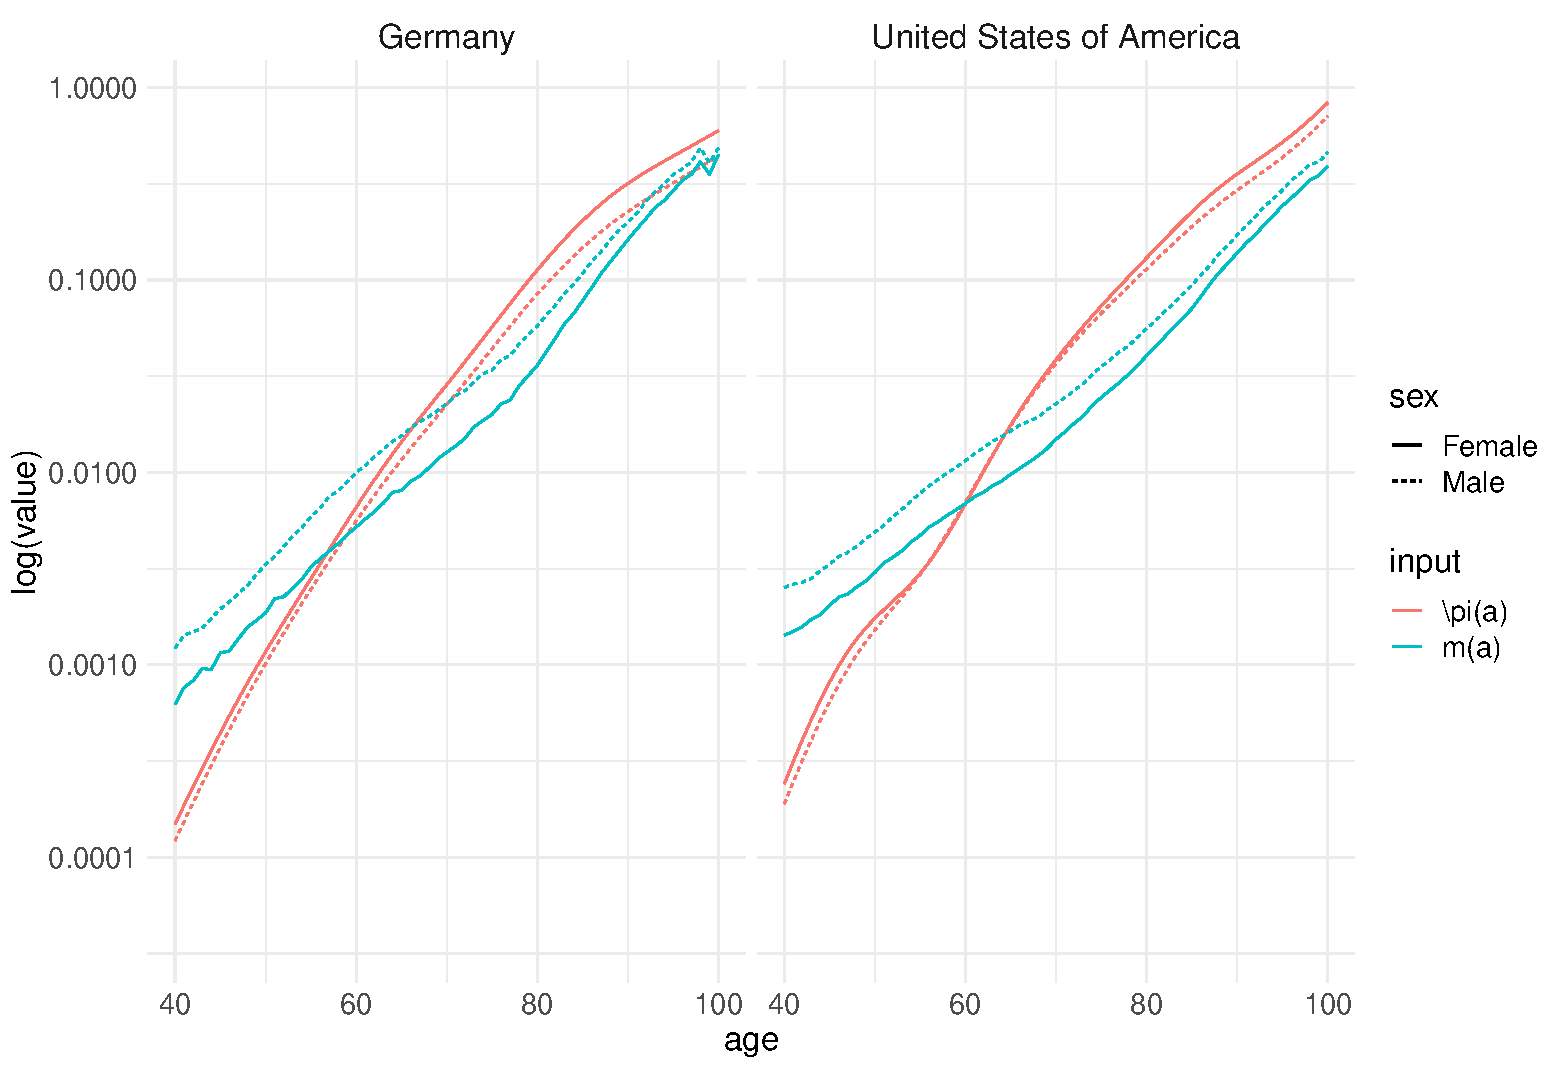
\includegraphics[width=0.5\textwidth]{fig1.pdf}
\end{figure}

We construct a hypothetical single-age pattern of the risk ratio of all-cause mortality of those with and without this condition. Our hypothetical age pattern of the risk ratio is based on the systematic review of \citet{liang2021mortality}, where a point estimate of 5.9 is stated as the average risk ratio, and studies such as \citet{james2014contribution} and \citet{garre2019survival}, which show that the risk ratio should diminish after age 70. We use a risk ratio pattern defined by the following polynomial equation over ages 0 to 100, shown also in Fig \ref{fig:Ra}:

\begin{equation}
R(a) = 7.964 + .01411  a -.0002017  a ^ 2 + -.000005974  a^3 \mathrm{.}
\end{equation}

\begin{figure}[ht!]
\centering
\caption{Risk ratio pattern $R(a)$ assumed}
\label{fig:Ra}
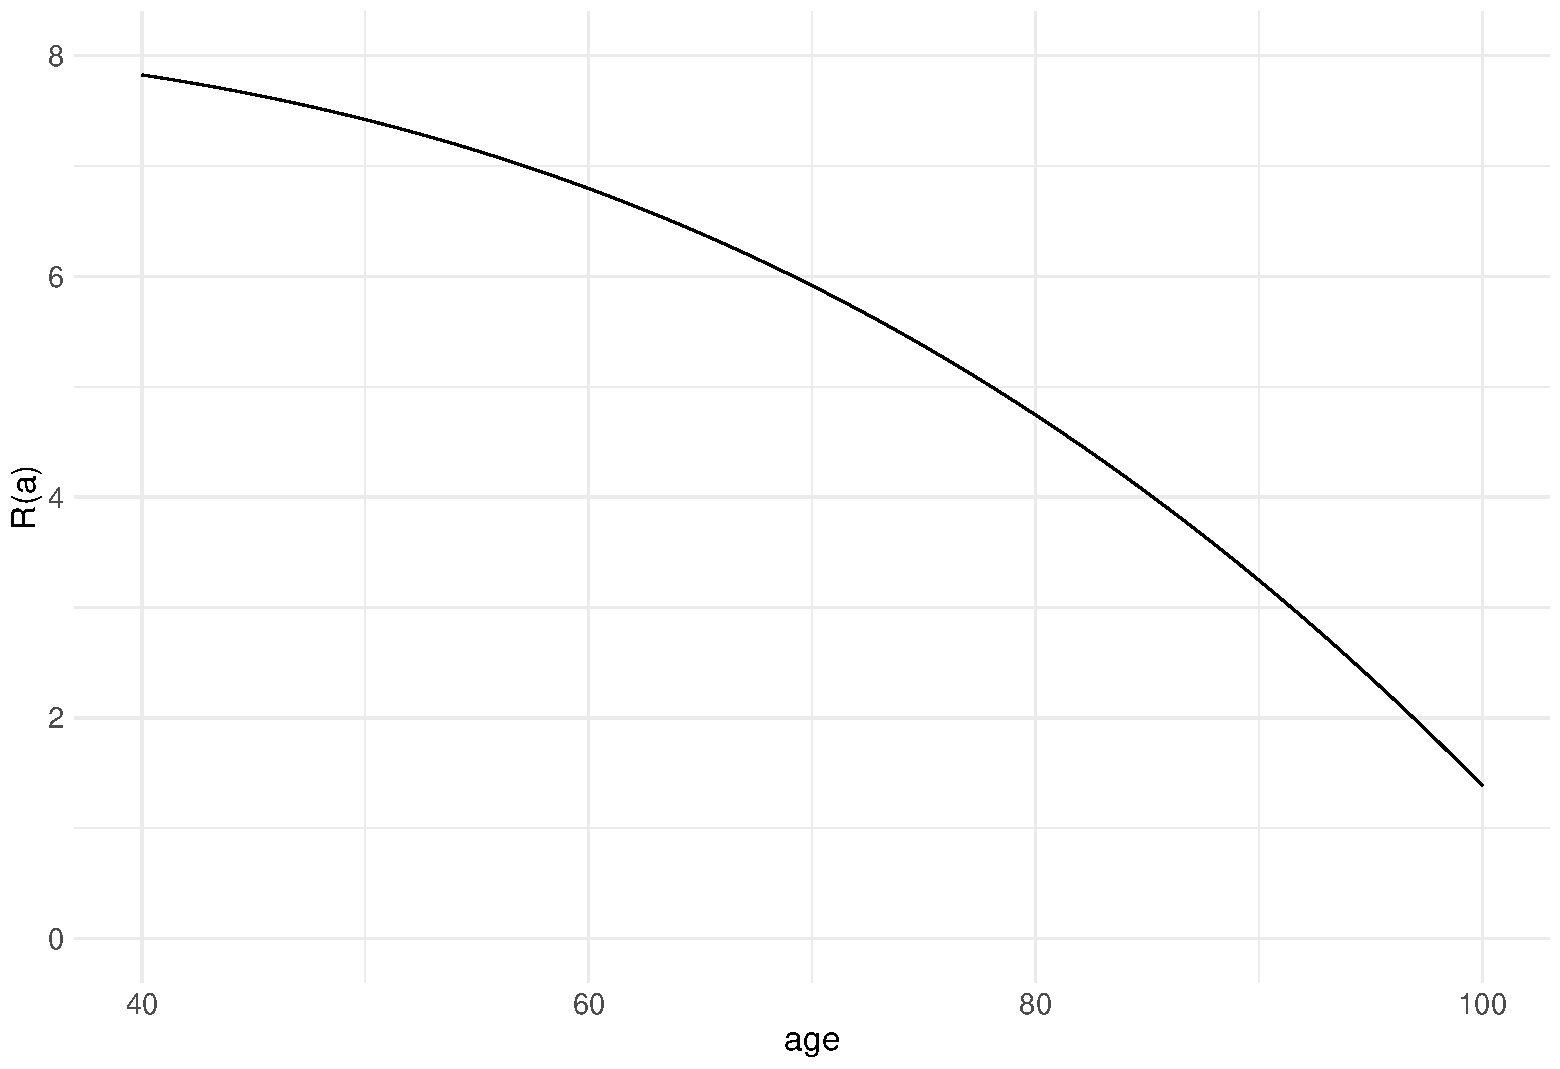
\includegraphics[width=0.5\textwidth]{fig2.pdf}
\end{figure}

This pattern will be the primary object of sensitivity analysis as this paper develops. As it stands, assuming a flat value of 5.9 for $R$ makes no obvious difference in the visualized results. 

\subsection{Results}\label{results}
Following equations \eqref{eq:mua} and \eqref{eq:mha}, we derive the following two conditional death probabilities $q^h(a)$ and $q^u(a)$, compared with the original lifetable death probabilities $q(a)$ (converted to be consistent with eq \eqref{eq:mx2lx}) in Fig \ref{fig:derived_rates}. We also include onset $p^{h\rightarrow u}(a)$ (red line) derived from eq \eqref{eq:onset}.

\begin{figure}[ht!]
\centering
\caption{Derived all-cause conditional mortality probabilities ($q^h(a)$,$q^u(a)$) by dementia status compared with original HMD lifetable ($q(a)$), as well as derived onset $p^{h \rightarrow u}(a)$.}
\label{fig:derived_rates}
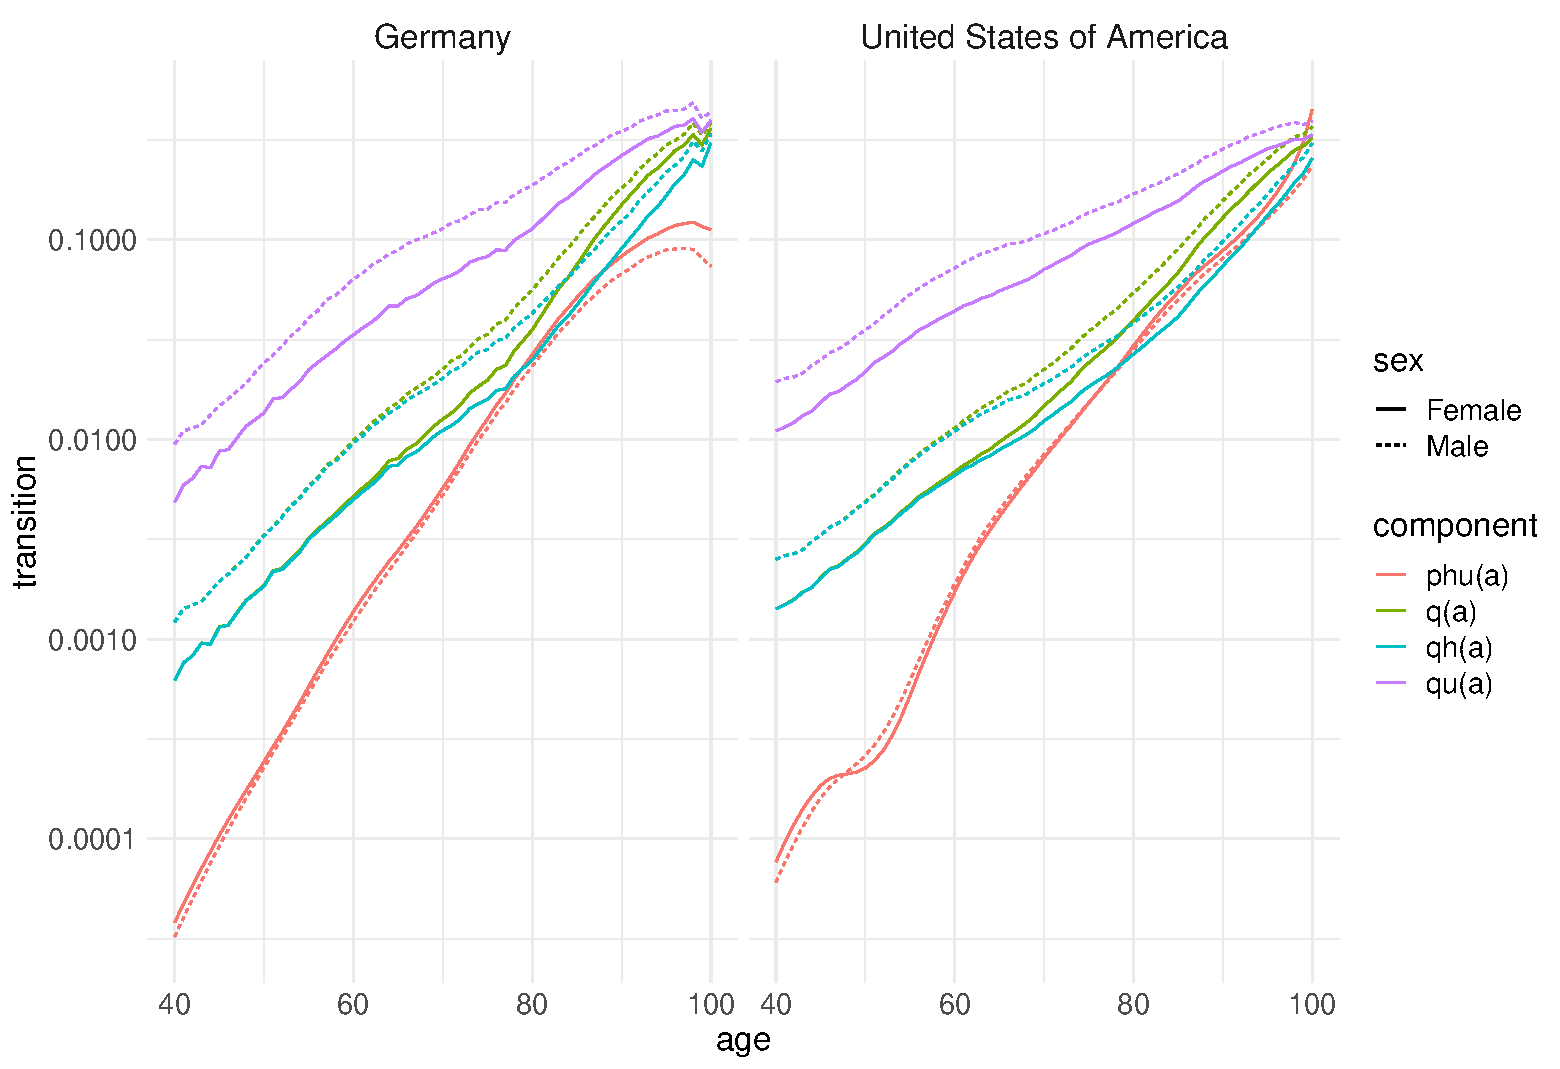
\includegraphics[width=0.5\textwidth]{fig3.pdf}
\end{figure}

Both the transitions in Fig \ref{fig:derived_rates} and the Sullivan inputs in Fig \ref{fig:sull_inputs} give the same expectancies at age 40, displayed in Table \ref{tab:expect}.

\begin{table}[ht!]
\caption{Remaining life expectancy at age 40 without (HLE) and with (ULE) dementia including Alzheimer's disease.}
\label{tab:expect}
\centering
\begin{tabular}{llrr}
  \hline
 country & sex & HLE & ULE \\ 
  \hline
Germany & Female & 41.78 & 2.15 \\ 
Germany & Male & 38.47 & 1.11 \\ 
United States of America & Female & 40.30 & 2.49 \\ 
United States of America & Male & 37.27 & 1.57 \\ 
   \hline
\end{tabular}
\end{table}

Finally, we show the results of incidence-based decomposition of sex differences in HLE, ULE, and total life expectancy, comparing results obtained when we calculate HLE using the Sullivan parameters of Fig \ref{fig:sull_inputs} versus the incidence parameters of Fig \ref{fig:derived_rates}.

\begin{table}[ht!]
\label{tab:results}
\caption{Comparison of decomposition approaches for sex differences in remaining life expectancy at age 40 with and without Dementia. }
\centering
\begin{tabular}{ll|rrrr|rr}
  
  \multicolumn{2}{c}{} & \multicolumn{4}{c}{Incidence} & \multicolumn{2}{c}{Sullivan} \\
  \hline
 Country & Expectancy & $\pi(40)$ & $p^{h\rightarrow u}$ & $q^h$ & $q^u$ & $m$ & $\pi$ \\ 
  \hline
Germany & HLE & -0.00 & -0.34 & 3.62 & 0.03 & 3.78 & -0.46 \\ 
Germany & ULE & 0.00 & 0.16 & 0.41 & 0.49 & 0.59 & 0.46 \\ 
Germany & Total & -0.00 & -0.19 & 4.03 & 0.51 & 4.36 & 0.00 \\ 
  \hline
United States of America & HLE & -0.00 & -0.04 & 3.04 & 0.02 & 3.31 & -0.28 \\ 
United States of America & ULE & 0.00 & 0.03 & 0.41 & 0.48 & 0.64 & 0.28 \\ 
United States of America & Total & -0.00 & -0.02 & 3.45 & 0.51 & 3.95 & 0.00 \\ 
   \hline
\end{tabular}
\end{table}

The main findings are that (i) initial conditions at age 40 play a negligible role in this data, (ii) males' lower onset of dementia in Germany reduced the sex-gap in HLE by around 4 months, and the overall life expectancy gap by 2 months, whereas in the USA sex differences in onset were negligible, (iii) most of the female advantage in all expectancies (HLE, ULE, Total LE) are due to lower mortality rates among those without dementia, accounting for over 3 years of the HLE and Total LE gaps in both countries, and almost 5 months of the ULE gap, (iv) higher male mortality rates among those with dementia increased the sex gap in ULE and Total LE by around half a year in both countries.

The Sullivan results are different in a few key ways: (i) with the exception of ULE in the USA, more weight is given to mortality for ULE and HLE (ii) the health effect for HLE ($\pi$) is symmetrical to that of ULE, whereas for the incidence-based decomposition onset ($p^{h\rightarrow u}$)  is not, (iii) the prevalence effect is of greater magnitude than the onset transition effect for both expectancies and countries, (iv) 100\% of the Total LE difference is attributed to mortality differences by necessity, in essence because the Sullivan approach gives the same mortality to both health states.

\section{Discussion}
These preliminary results highlight how incidence-based decomposition can yield more specific insights into what explains differences in HLE, ULE and Total LE. In this current proposal, we include a health condition with a very large lethality penalty. We will add another example of a non-reversible health condition with a different prevalence pattern and different likely rate ratio that might highlight other ways that this method gives more information. For example, in the current dementia example, initial conditions at age 40 were unimportant, but in general we'd expect initial conditions to be very important for multistate models with non-reversible states of decreased health.

We think that leveraging the rate ratio as we do here could be a useful trick for other empirical exercises. For example, when estimating multistate transitions from surveys like HRS, one can adjust for mortality underestimation using the directly derived rate ratio and an a higher quality lifetable based on vital statistics. We have not yet reflected on what further minimal assumption would be required in order to extend the method to include recovery transitions.

\section{Tables}\label{sec5}

Tables can be inserted via the normal table and tabular environment. To put
footnotes inside tables you should use \verb+\footnotetext[]{...}+ tag.
The footnote appears just below the table itself (refer Tables~\ref{tab1} and \ref{tab2}). 
For the corresponding footnotemark use \verb+\footnotemark[...]+

\begin{table}[h]
\caption{Caption text}\label{tab1}%
\begin{tabular}{@{}llll@{}}
\toprule
Column 1 & Column 2  & Column 3 & Column 4\\
\midrule
row 1    & data 1   & data 2  & data 3  \\
row 2    & data 4   & data 5\footnotemark[1]  & data 6  \\
row 3    & data 7   & data 8  & data 9\footnotemark[2]  \\
\botrule
\end{tabular}
\footnotetext{Source: This is an example of table footnote. This is an example of table footnote.}
\footnotetext[1]{Example for a first table footnote. This is an example of table footnote.}
\footnotetext[2]{Example for a second table footnote. This is an example of table footnote.}
\end{table}

\noindent
The input format for the above table is as follows:

%%=============================================%%
%% For presentation purpose, we have included  %%
%% \bigskip command. please ignore this.       %%
%%=============================================%%
\bigskip
\begin{verbatim}
\begin{table}[<placement-specifier>]
\caption{<table-caption>}\label{<table-label>}%
\begin{tabular}{@{}llll@{}}
\toprule
Column 1 & Column 2 & Column 3 & Column 4\\
\midrule
row 1 & data 1 & data 2	 & data 3 \\
row 2 & data 4 & data 5\footnotemark[1] & data 6 \\
row 3 & data 7 & data 8	 & data 9\footnotemark[2]\\
\botrule
\end{tabular}
\footnotetext{Source: This is an example of table footnote. 
This is an example of table footnote.}
\footnotetext[1]{Example for a first table footnote.
This is an example of table footnote.}
\footnotetext[2]{Example for a second table footnote. 
This is an example of table footnote.}
\end{table}
\end{verbatim}
\bigskip
%%=============================================%%
%% For presentation purpose, we have included  %%
%% \bigskip command. please ignore this.       %%
%%=============================================%%

\begin{table}[h]
\caption{Example of a lengthy table which is set to full textwidth}\label{tab2}
\begin{tabular*}{\textwidth}{@{\extracolsep\fill}lcccccc}
\toprule%
& \multicolumn{3}{@{}c@{}}{Element 1\footnotemark[1]} & \multicolumn{3}{@{}c@{}}{Element 2\footnotemark[2]} \\\cmidrule{2-4}\cmidrule{5-7}%
Project & Energy & $\sigma_{calc}$ & $\sigma_{expt}$ & Energy & $\sigma_{calc}$ & $\sigma_{expt}$ \\
\midrule
Element 3  & 990 A & 1168 & $1547\pm12$ & 780 A & 1166 & $1239\pm100$\\
Element 4  & 500 A & 961  & $922\pm10$  & 900 A & 1268 & $1092\pm40$\\
\botrule
\end{tabular*}
\footnotetext{Note: This is an example of table footnote. This is an example of table footnote this is an example of table footnote this is an example of~table footnote this is an example of table footnote.}
\footnotetext[1]{Example for a first table footnote.}
\footnotetext[2]{Example for a second table footnote.}
\end{table}

\vfill\eject

In case of double column layout, tables which do not fit in single column width should be set to full text width. For this, you need to use \verb+\begin{table*}+ \verb+...+ \verb+\end{table*}+ instead of \verb+\begin{table}+ \verb+...+ \verb+\end{table}+ environment. Lengthy tables which do not fit in textwidth should be set as rotated table. For this, you need to use \verb+\begin{sidewaystable}+ \verb+...+ \verb+\end{sidewaystable}+ instead of \verb+\begin{table*}+ \verb+...+ \verb+\end{table*}+ environment. This environment puts tables rotated to single column width. For tables rotated to double column width, use \verb+\begin{sidewaystable*}+ \verb+...+ \verb+\end{sidewaystable*}+.

\begin{sidewaystable}
\caption{Tables which are too long to fit, should be written using the ``sidewaystable'' environment as shown here}\label{tab3}
\begin{tabular*}{\textheight}{@{\extracolsep\fill}lcccccc}
\toprule%
& \multicolumn{3}{@{}c@{}}{Element 1\footnotemark[1]}& \multicolumn{3}{@{}c@{}}{Element\footnotemark[2]} \\\cmidrule{2-4}\cmidrule{5-7}%
Projectile & Energy	& $\sigma_{calc}$ & $\sigma_{expt}$ & Energy & $\sigma_{calc}$ & $\sigma_{expt}$ \\
\midrule
Element 3 & 990 A & 1168 & $1547\pm12$ & 780 A & 1166 & $1239\pm100$ \\
Element 4 & 500 A & 961  & $922\pm10$  & 900 A & 1268 & $1092\pm40$ \\
Element 5 & 990 A & 1168 & $1547\pm12$ & 780 A & 1166 & $1239\pm100$ \\
Element 6 & 500 A & 961  & $922\pm10$  & 900 A & 1268 & $1092\pm40$ \\
\botrule
\end{tabular*}
\footnotetext{Note: This is an example of table footnote this is an example of table footnote this is an example of table footnote this is an example of~table footnote this is an example of table footnote.}
\footnotetext[1]{This is an example of table footnote.}
\end{sidewaystable}

\section{Figures}\label{sec6}

As per the \LaTeX\ standards you need to use eps images for \LaTeX\ compilation and \verb+pdf/jpg/png+ images for \verb+PDFLaTeX+ compilation. This is one of the major difference between \LaTeX\ and \verb+PDFLaTeX+. Each image should be from a single input .eps/vector image file. Avoid using subfigures. The command for inserting images for \LaTeX\ and \verb+PDFLaTeX+ can be generalized. The package used to insert images in \verb+LaTeX/PDFLaTeX+ is the graphicx package. Figures can be inserted via the normal figure environment as shown in the below example:

%%=============================================%%
%% For presentation purpose, we have included  %%
%% \bigskip command. please ignore this.       %%
%%=============================================%%
\bigskip
\begin{verbatim}
\begin{figure}[<placement-specifier>]
\centering
\includegraphics{<eps-file>}
\caption{<figure-caption>}\label{<figure-label>}
\end{figure}
\end{verbatim}
\bigskip
%%=============================================%%
%% For presentation purpose, we have included  %%
%% \bigskip command. please ignore this.       %%
%%=============================================%%

%\begin{figure}[h]%
%\centering
%\includegraphics[width=0.9\textwidth]{fig.eps}
%\caption{This is a widefig. This is an example of long caption this is an example of long caption  this is an example of long caption this is an example of long caption}\label{fig1}
%\end{figure}

%In case of double column layout, the above format puts figure captions/images to single column width. To get spanned images, we need to provide \verb+\begin{figure*}+ \verb+...+ \verb+\end{figure*}+.

%For sample purpose, we have included the width of images in the optional argument of \verb+\includegraphics+ tag. Please ignore this. 

%\section{Algorithms, Program codes and Listings}\label{sec7}

%Packages \verb+algorithm+, \verb+algorithmicx+ and \verb+algpseudocode+ are used for setting algorithms in \LaTeX\ using the format:

%%=============================================%%
%% For presentation purpose, we have included  %%
%% \bigskip command. please ignore this.       %%
%%=============================================%%
%\bigskip
%\begin{verbatim}
%\begin{algorithm}
%\caption{<alg-caption>}\label{<alg-label>}
%\begin{algorithmic}[1]
%. . .
%\end{algorithmic}
%\end{algorithm}
%\end{verbatim}
%\bigskip
%%=============================================%%
%% For presentation purpose, we have included  %%
%% \bigskip command. please ignore this.       %%
%%=============================================%%

%You may refer above listed package documentations for more details before setting \verb+algorithm+ environment. For program codes, the ``verbatim'' package is required and the command to be used is \verb+\begin{verbatim}+ \verb+...+ \verb+\end{verbatim}+. 

%Similarly, for \verb+listings+, use the \verb+listings+ package. \verb+\begin{lstlisting}+ \verb+...+ \verb+\end{lstlisting}+ is used to set environments similar to \verb+verbatim+ environment. Refer to the \verb+lstlisting+ package documentation for more details.

%A fast exponentiation procedure:

%\lstset{texcl=true,basicstyle=\small\sf,commentstyle=\small\rm,mathescape=true,escapeinside={(*}{*)}}
%\begin{lstlisting}
%begin
%  for $i:=1$ to $10$ step $1$ do
%      expt($2,i$);  
%      newline() od                (*\textrm{Comments will be set flush to the right margin}*)
%where
%proc expt($x,n$) $\equiv$
%  $z:=1$;
%  do if $n=0$ then exit fi;
%     do if odd($n$) then exit fi;                 
%        comment: (*\textrm{This is a comment statement;}*)
%        $n:=n/2$; $x:=x*x$ od;
%     { $n>0$ };
%     $n:=n-1$; $z:=z*x$ od;
%  print($z$). 
%end
%\end{lstlisting}

%\begin{algorithm}
%\caption{Calculate $y = x^n$}\label{algo1}
%\begin{algorithmic}[1]
%\Require $n \geq 0 \vee x \neq 0$
%\Ensure $y = x^n$ 
%\State $y \Leftarrow 1$
%\If{$n < 0$}\label{algln2}
%        \State $X \Leftarrow 1 / x$
%        \State $N \Leftarrow -n$
%\Else
%        \State $X \Leftarrow x$
%        \State $N \Leftarrow n$
%\EndIf
%\While{$N \neq 0$}
%        \If{$N$ is even}
%            \State $X \Leftarrow X \times X$
%            \State $N \Leftarrow N / 2$
%        \Else[$N$ is odd]
%            \State $y \Leftarrow y \times X$
%            \State $N \Leftarrow N - 1$
%        \EndIf
%\EndWhile
%\end{algorithmic}
%\end{algorithm}

%%=============================================%%
%% For presentation purpose, we have included  %%
%% \bigskip command. please ignore this.       %%
%%=============================================%%
%\bigskip
%\begin{minipage}{\hsize}%
%\lstset{frame=single,framexleftmargin=-1pt,framexrightmargin=-17pt,framesep=12pt,linewidth=0.98\textwidth,language=pascal}% Set your language (you can change the language for each code-block optionally)
%%%% Start your code-block
%\begin{lstlisting}
%for i:=maxint to 0 do
%begin
%{ do nothing }
%end;
%Write('Case insensitive ');
%Write('Pascal keywords.');
%\end{lstlisting}
%\end{minipage}
%
%\section{Cross referencing}\label{sec8}
%
%Environments such as figure, table, equation and align can have a label
%declared via the \verb+\label{#label}+ command. For figures and table
%environments use the \verb+\label{}+ command inside or just
%below the \verb+\caption{}+ command. You can then use the
%\verb+\ref{#label}+ command to cross-reference them. As an example, consider
%the label declared for Figure~\ref{fig1} which is
%\verb+\label{fig1}+. To cross-reference it, use the command 
%\verb+Figure \ref{fig1}+, for which it comes up as
%``Figure~\ref{fig1}''. 
%
%To reference line numbers in an algorithm, consider the label declared for the line number 2 of Algorithm~\ref{algo1} is \verb+\label{algln2}+. To cross-reference it, use the command \verb+\ref{algln2}+ for which it comes up as line~\ref{algln2} of Algorithm~\ref{algo1}.
%
%\subsection{Details on reference citations}\label{subsec7}
%
%Standard \LaTeX\ permits only numerical citations. To support both numerical and author-year citations this template uses \verb+natbib+ \LaTeX\ package. For style guidance please refer to the template user manual.
%
%Here is an example for \verb+\cite{...}+: \cite{bib1}. Another example for \verb+\citep{...}+: \citep{bib2}. For author-year citation mode, \verb+\cite{...}+ prints Jones et al. (1990) and \verb+\citep{...}+ prints (Jones et al., 1990).
%
%All cited bib entries are printed at the end of this article: \cite{bib3}, \cite{bib4}, \cite{bib5}, \cite{bib6}, \cite{bib7}, \cite{bib8}, \cite{bib9}, \cite{bib10}, \cite{bib11}, \cite{bib12} and \cite{bib13}.

%\section{Examples for theorem like environments}\label{sec10}
%
%For theorem like environments, we require \verb+amsthm+ package. There are three types of predefined theorem styles exists---\verb+thmstyleone+, \verb+thmstyletwo+ and \verb+thmstylethree+ 
%
%%%=============================================%%
%%% For presentation purpose, we have included  %%
%%% \bigskip command. please ignore this.       %%
%%%=============================================%%
%\bigskip
%\begin{tabular}{|l|p{19pc}|}
%\hline
%\verb+thmstyleone+ & Numbered, theorem head in bold font and theorem text in italic style \\\hline
%\verb+thmstyletwo+ & Numbered, theorem head in roman font and theorem text in italic style \\\hline
%\verb+thmstylethree+ & Numbered, theorem head in bold font and theorem text in roman style \\\hline
%\end{tabular}
%\bigskip
%%%=============================================%%
%%% For presentation purpose, we have included  %%
%%% \bigskip command. please ignore this.       %%
%%%=============================================%%
%
%For mathematics journals, theorem styles can be included as shown in the following examples:

%\begin{theorem}[Theorem subhead]\label{thm1}
%Example theorem text. Example theorem text. Example theorem text. Example theorem text. Example theorem text. 
%Example theorem text. Example theorem text. Example theorem text. Example theorem text. Example theorem text. 
%Example theorem text. 
%\end{theorem}
%
%Sample body text. Sample body text. Sample body text. Sample body text. Sample body text. Sample body text. Sample body text. Sample body text.
%
%\begin{proposition}
%Example proposition text. Example proposition text. Example proposition text. Example proposition text. Example proposition text. 
%Example proposition text. Example proposition text. Example proposition text. Example proposition text. Example proposition text. 
%\end{proposition}
%
%Sample body text. Sample body text. Sample body text. Sample body text. Sample body text. Sample body text. Sample body text. Sample body text.
%
%\begin{example}
%Phasellus adipiscing semper elit. Proin fermentum massa
%ac quam. Sed diam turpis, molestie vitae, placerat a, molestie nec, leo. Maecenas lacinia. Nam ipsum ligula, eleifend
%at, accumsan nec, suscipit a, ipsum. Morbi blandit ligula feugiat magna. Nunc eleifend consequat lorem. 
%\end{example}
%
%Sample body text. Sample body text. Sample body text. Sample body text. Sample body text. Sample body text. Sample body text. Sample body text.
%
%\begin{remark}
%Phasellus adipiscing semper elit. Proin fermentum massa
%ac quam. Sed diam turpis, molestie vitae, placerat a, molestie nec, leo. Maecenas lacinia. Nam ipsum ligula, eleifend
%at, accumsan nec, suscipit a, ipsum. Morbi blandit ligula feugiat magna. Nunc eleifend consequat lorem. 
%\end{remark}
%
%Sample body text. Sample body text. Sample body text. Sample body text. Sample body text. Sample body text. Sample body text. Sample body text.
%
%\begin{definition}[Definition sub head]
%Example definition text. Example definition text. Example definition text. Example definition text. Example definition text. Example definition text. Example definition text. Example definition text. 
%\end{definition}

%Additionally a predefined ``proof'' environment is available: \verb+\begin{proof}+ \verb+...+ \verb+\end{proof}+. This prints a ``Proof'' head in italic font style and the ``body text'' in roman font style with an open square at the end of each proof environment. 
%
%\begin{proof}
%Example for proof text. Example for proof text. Example for proof text. Example for proof text. Example for proof text. Example for proof text. Example for proof text. Example for proof text. Example for proof text. Example for proof text. 
%\end{proof}
%
%Sample body text. Sample body text. Sample body text. Sample body text. Sample body text. Sample body text. Sample body text. Sample body text.
%
%\begin{proof}[Proof of Theorem~{\upshape\ref{thm1}}]
%Example for proof text. Example for proof text. Example for proof text. Example for proof text. Example for proof text. Example for proof text. Example for proof text. Example for proof text. Example for proof text. Example for proof text. 
%\end{proof}

%\noindent
%For a quote environment, use \verb+\begin{quote}...\end{quote}+
%\begin{quote}
%Quoted text example. Aliquam porttitor quam a lacus. Praesent vel arcu ut tortor cursus volutpat. In vitae pede quis diam bibendum placerat. Fusce elementum
%convallis neque. Sed dolor orci, scelerisque ac, dapibus nec, ultricies ut, mi. Duis nec dui quis leo sagittis commodo.
%\end{quote}
%
%Sample body text. Sample body text. Sample body text. Sample body text. Sample body text (refer Figure~\ref{fig1}). Sample body text. Sample body text. Sample body text (refer Table~\ref{tab3}). 
%
%\section{Methods}\label{sec11}
%
%Topical subheadings are allowed. Authors must ensure that their Methods section includes adequate experimental and characterization data necessary for others in the field to reproduce their work. Authors are encouraged to include RIIDs where appropriate. 

%\textbf{Ethical approval declarations} (only required where applicable) Any article reporting experiment/s carried out on (i)~live vertebrate (or higher invertebrates), (ii)~humans or (iii)~human samples must include an unambiguous statement within the methods section that meets the following requirements: 

%\begin{enumerate}[1.]
%\item Approval: a statement which confirms that all experimental protocols were approved by a named institutional and/or licensing committee. Please identify the approving body in the methods section

%\item Accordance: a statement explicitly saying that the methods were carried out in accordance with the relevant guidelines and regulations

%\item Informed consent (for experiments involving humans or human tissue samples): include a statement confirming that informed consent was obtained from all participants and/or their legal guardian/s
%\end{enumerate}

%If your manuscript includes potentially identifying patient/participant information, or if it describes human transplantation research, or if it reports results of a clinical trial then  additional information will be required. Please visit (\url{https://www.nature.com/nature-research/editorial-policies}) for Nature Portfolio journals, (\url{https://www.springer.com/gp/authors-editors/journal-author/journal-author-helpdesk/publishing-ethics/14214}) for Springer Nature journals, or (\url{https://www.biomedcentral.com/getpublished/editorial-policies\#ethics+and+consent}) for BMC.

\section{Discussion}\label{sec12}

Discussions should be brief and focused. In some disciplines use of Discussion or `Conclusion' is interchangeable. It is not mandatory to use both. Some journals prefer a section `Results and Discussion' followed by a section `Conclusion'. Please refer to Journal-level guidance for any specific requirements. 

\section{Conclusion}\label{sec13}

Conclusions may be used to restate your hypothesis or research question, restate your major findings, explain the relevance and the added value of your work, highlight any limitations of your study, describe future directions for research and recommendations. 

In some disciplines use of Discussion or 'Conclusion' is interchangeable. It is not mandatory to use both. Please refer to Journal-level guidance for any specific requirements. 

\backmatter

\bmhead{Supplementary information}

If your article has accompanying supplementary file/s please state so here. 

Authors reporting data from electrophoretic gels and blots should supply the full unprocessed scans for key as part of their Supplementary information. This may be requested by the editorial team/s if it is missing.

Please refer to Journal-level guidance for any specific requirements.

\bmhead{Acknowledgments}

Acknowledgments are not compulsory. Where included they should be brief. Grant or contribution numbers may be acknowledged.

Please refer to Journal-level guidance for any specific requirements.

\section*{Declarations}

Some journals require declarations to be submitted in a standardised format. Please check the Instructions for Authors of the journal to which you are submitting to see if you need to complete this section. If yes, your manuscript must contain the following sections under the heading `Declarations':

\begin{itemize}
\item Funding
\item Conflict of interest/Competing interests (check journal-specific guidelines for which heading to use)
\item Ethics approval 
\item Consent to participate
\item Consent for publication
\item Availability of data and materials
\item Code availability 
\item Authors' contributions
\end{itemize}

\noindent
If any of the sections are not relevant to your manuscript, please include the heading and write `Not applicable' for that section. 

%%===================================================%%
%% For presentation purpose, we have included        %%
%% \bigskip command. please ignore this.             %%
%%===================================================%%
\bigskip
\begin{flushleft}%
Editorial Policies for:

\bigskip\noindent
Springer journals and proceedings: \url{https://www.springer.com/gp/editorial-policies}

\bigskip\noindent
Nature Portfolio journals: \url{https://www.nature.com/nature-research/editorial-policies}

\bigskip\noindent
\textit{Scientific Reports}: \url{https://www.nature.com/srep/journal-policies/editorial-policies}

\bigskip\noindent
BMC journals: \url{https://www.biomedcentral.com/getpublished/editorial-policies}
\end{flushleft}

\begin{appendices}

\section{Section title of first appendix}\label{secA1}

An appendix contains supplementary information that is not an essential part of the text itself but which may be helpful in providing a more comprehensive understanding of the research problem or it is information that is too cumbersome to be included in the body of the paper.

%%=============================================%%
%% For submissions to Nature Portfolio Journals %%
%% please use the heading ``Extended Data''.   %%
%%=============================================%%

%%=============================================================%%
%% Sample for another appendix section			       %%
%%=============================================================%%

%% \section{Example of another appendix section}\label{secA2}%
%% Appendices may be used for helpful, supporting or essential material that would otherwise 
%% clutter, break up or be distracting to the text. Appendices can consist of sections, figures, 
%% tables and equations etc.

\end{appendices}

%%===========================================================================================%%
%% If you are submitting to one of the Nature Portfolio journals, using the eJP submission   %%
%% system, please include the references within the manuscript file itself. You may do this  %%
%% by copying the reference list from your .bbl file, paste it into the main manuscript .tex %%
%% file, and delete the associated \verb+\bibliography+ commands.                            %%
%%===========================================================================================%%

\bibliography{references}% common bib file
%% if required, the content of .bbl file can be included here once bbl is generated
%%\input sn-article.bbl


\end{document}
